% !TeX root = ../main.tex
\documentclass[../main.tex]{subfiles}

\begin{document}

Nhóm đã tiến hành đánh giá hiệu năng tải của hệ thống thông qua công cụ Load Testing được cung cấp bởi Azure.
Hệ thống này sử dụng JMeter để mô phỏng việc gửi yêu cầu từ phía khách với số lượng lớn, đồng thời cung cấp các biểu đồ và số liệu trực quan để theo dõi tình trạng phía khách và hệ thống.
Bài kiểm tra được thiết lập với 50 người dùng đồng thời gửi liên tục các yêu cầu trong vòng 1 phút tới các API của hệ thống, bao gồm lấy thông tin người dùng, lấy bài viết ngẫu nhiên, lấy bình luận của bài viết và lấy các bài viết trên trang chủ.

Hệ thống được triển khai trên cấu hình B3 với 4 vCPU và 7GB RAM.
Cơ sở dữ liệu sử dụng hạng tiêu chuẩn với 1 vCore và 2 GB RAM, hỗ trợ tối đa 640 thao tác vào ra dữ liệu mỗi giây.
Bộ nhớ tạm Redis sử dụng cấu hình với 2 vCPU và 0.5GB bộ nhớ.

Dưới đây là một số kết quả thu được từ bài kiểm tra:

\begin{figure}[H]{Kết quả kiểm tra tải}
    \centering
    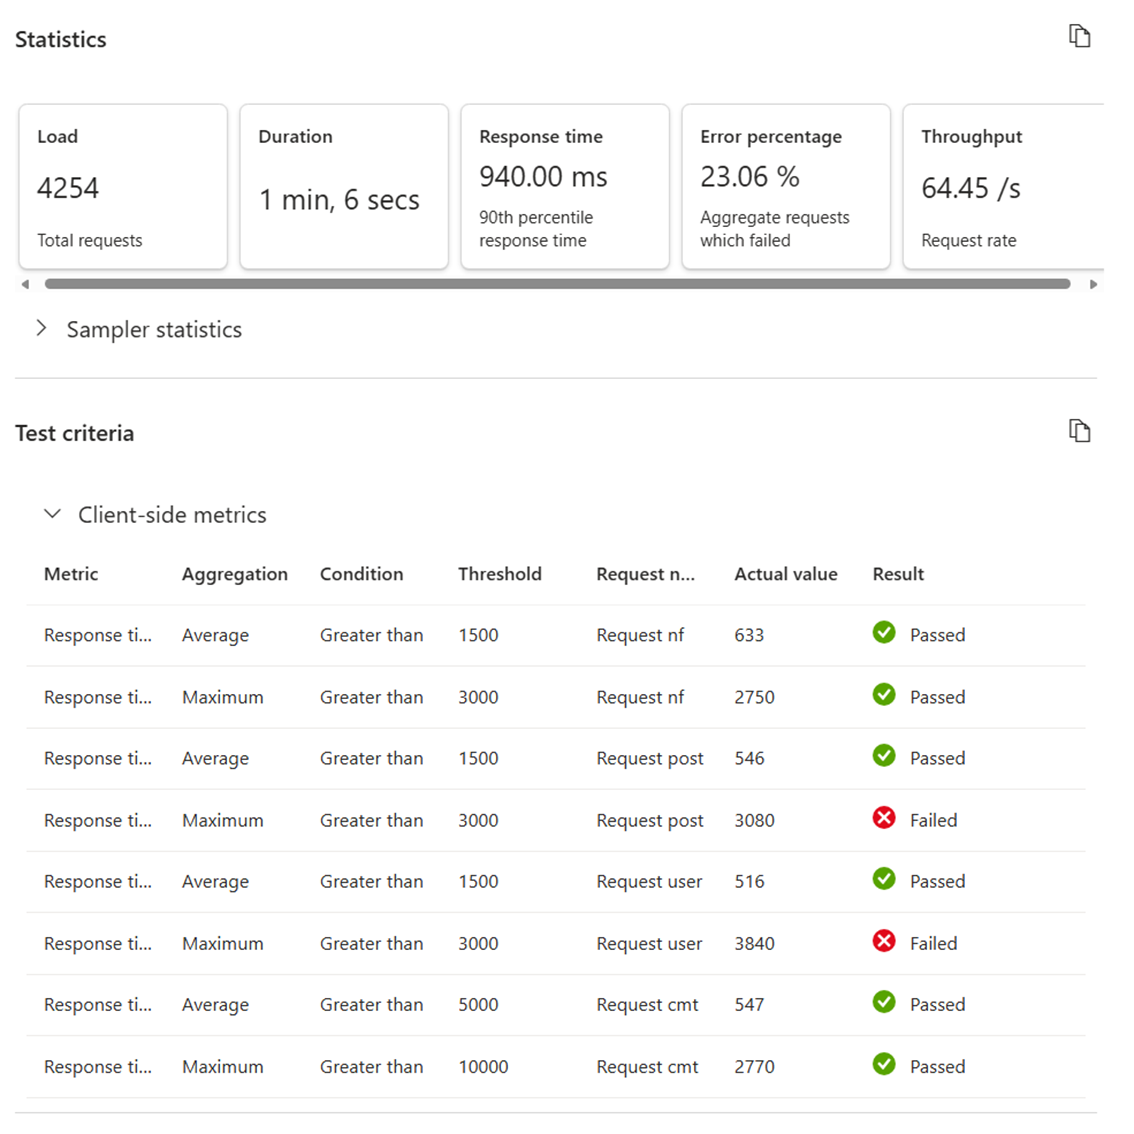
\includegraphics[width=0.9\textwidth]{loadtest_metric/stats.png}
    \label{fig:testresult}
\end{figure}

Trong 1 phút, hệ thống xử lí được hơn 4200 yêu cầu, với thông lượng khoảng 64 yêu cầu mỗi giây.
Thời gian phản hồi trung bình cho mỗi loại yêu cầu rơi vào khoảng từ 550ms đến 650ms. Thời gian phản hồi tối đa là gần 4 giây.
90\% các yêu cầu được phản hồi trong vòng dưới 1 giây, cho thấy hệ thống có khả năng chịu tải tương đối tốt với kịch bản sử dụng hiện tại, khi ứng dụng có lưu lượng truy cập thấp, rải rác vào các thời điểm và ít khi xảy ra cao điểm tắc nghẽn.

\begin{figure}[H]{Thống kê phía khách}
    \centering
    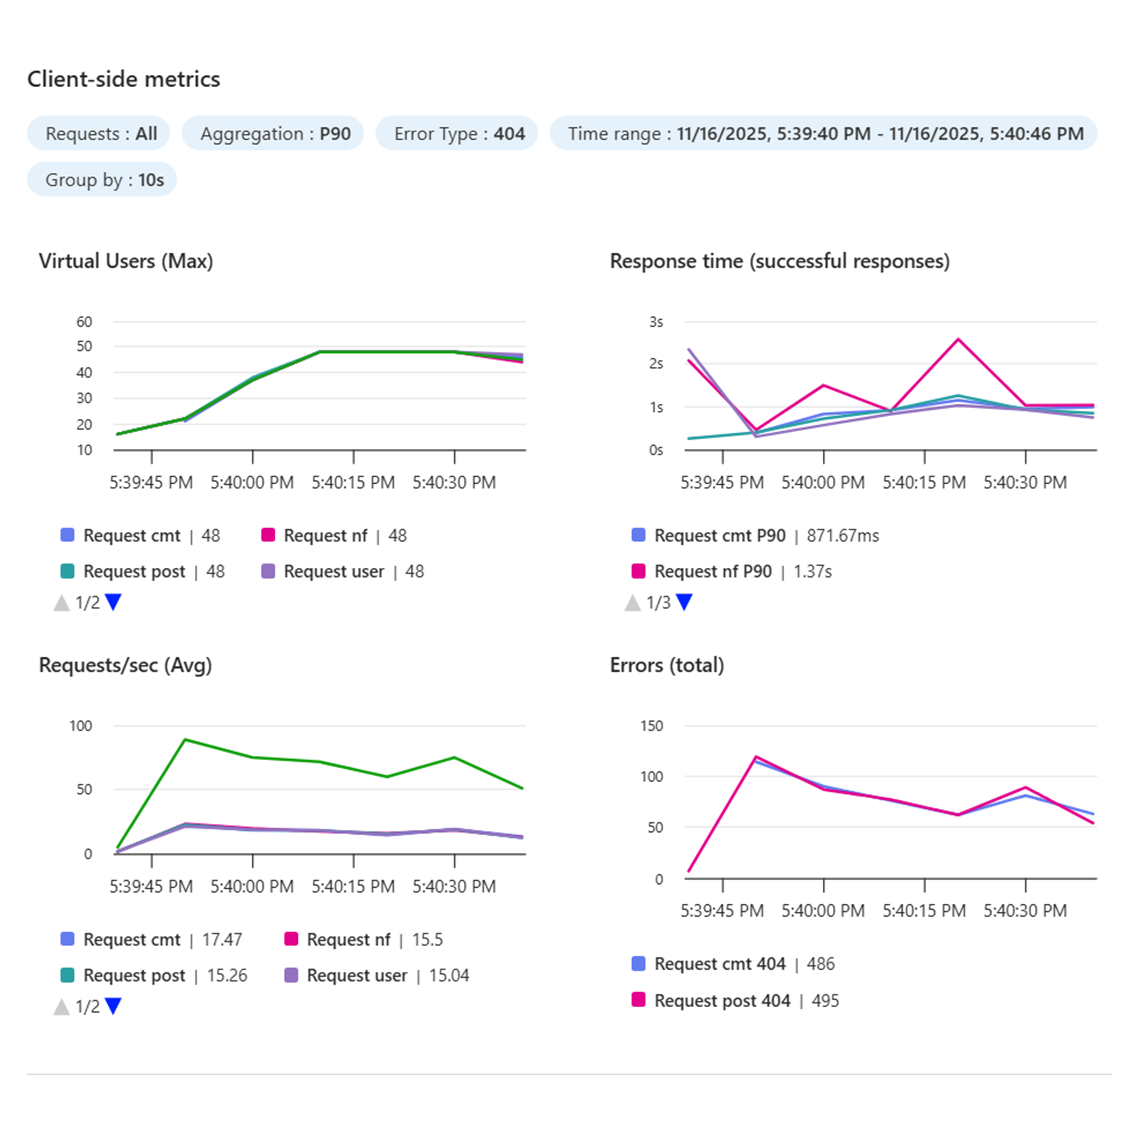
\includegraphics[width=0.9\textwidth]{loadtest_metric/client.png}
    \label{fig:clientmetrics}
\end{figure}

Bài kiểm tra thực hiện với số người dùng đồng thời tăng dần, và đạt tối đa ở 20 giây sau khi bắt đầu.
Trong thời gian đó, có thể thấy hệ thống xử lí được nhiều yêu cầu nhất trong một giây, đạt đỉnh ở mức gần 100 yêu cầu tải bài viết, và khoảng 20 yêu cầu mỗi loại khác.
Sau đó hệ thống dần đi vào trạng thái ổn định, biểu đồ có chút giảm nhẹ do số người dùng đồng thời đạt đỉnh.
Ở một số thời điểm, thời gian phản hồi thành công tăng vọt, do bộ nhớ tạm đã bị xóa, và các yêu cầu phải truy cập trực tiếp vào cơ sở dữ liệu, sau đó lại giảm xuống.
Về phần lỗi, hệ thống chỉ ghi nhận các lỗi về việc tài nguyên không tìm thấy (404) do các yêu cầu được tạo ngẫu nhiên.

\begin{figure}[H]{Thống kê phía máy chủ}
    \centering
    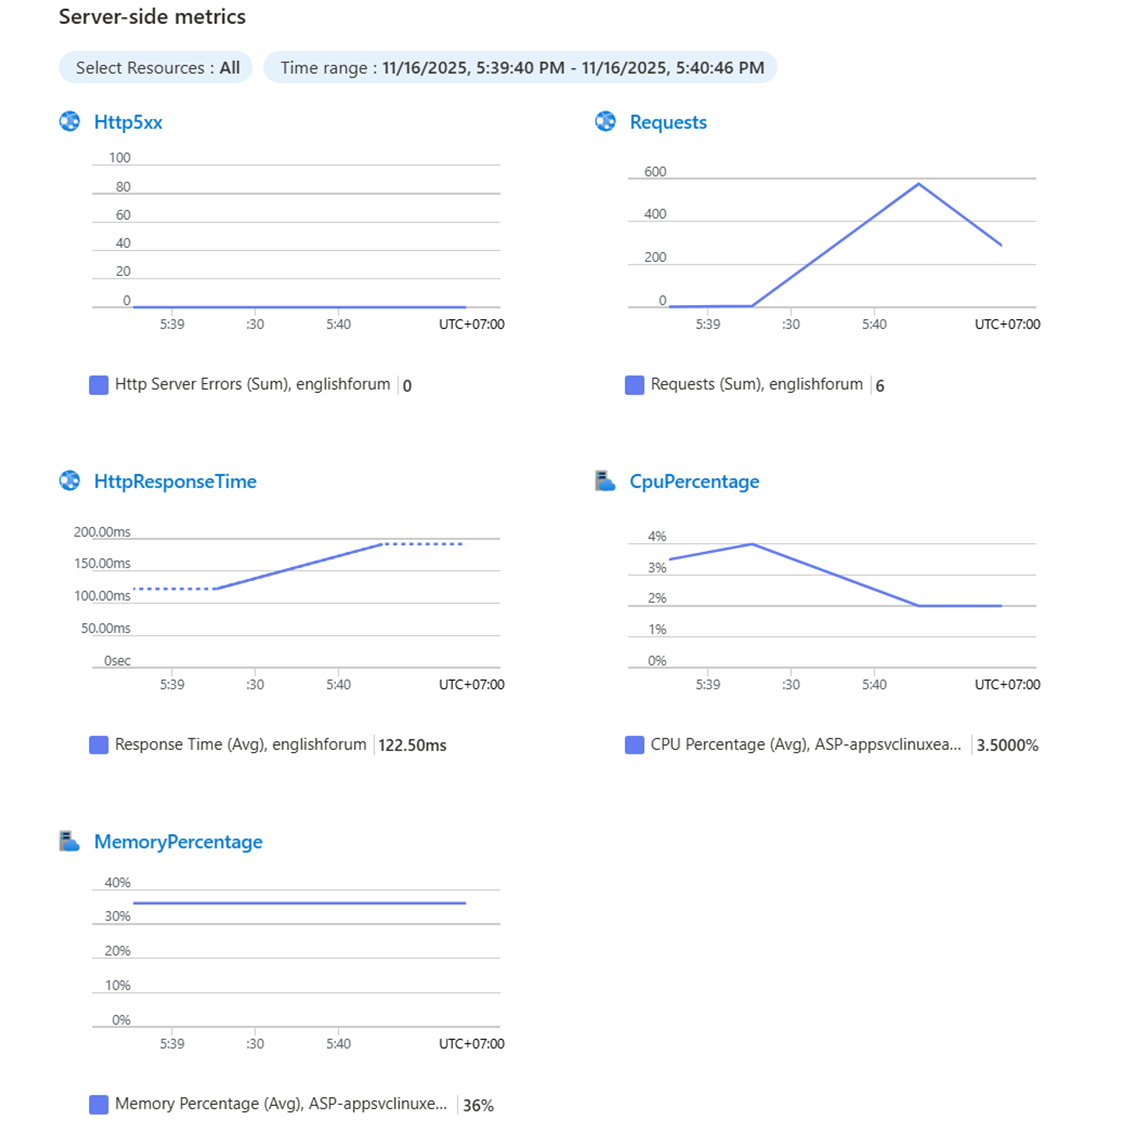
\includegraphics[width=0.9\textwidth]{loadtest_metric/server.png}
    \label{fig:servermetrics}
\end{figure}

Phía trên là biểu đồ theo dõi hoạt động của máy chủ. Nó cho thấy rằng hệ thống vẫn có khả năng xử lí thêm nhiều yêu cầu hơn nữa.
Trong quá trình chạy kiểm thử, không xảy ra lỗi hệ thống (Http5xx) nào, CPU và RAM dùng vẫn ở mức tương đối thấp.
Tuy nhiên nhóm cũng đã chạy thử với các kịch bản có số người dùng lớn hơn, và hệ thống không thể đáp ứng được sau một khoảng thời gian do tắc nghẽn ở hệ thống cơ sở dữ liệu.
Chi phí vận hành cơ sở dữ liệu và bộ nhớ đệm trên Azure tương đối cao, và với tình hình sử dụng hiện tại thì gói dịch vụ cơ bản là phù hợp nhất cho hệ thống.

\end{document}